\documentclass[hidelinks]{ctexart}

\usepackage{van-de-la-illinoise}
\usepackage{cmbright}
\usepackage{nccmath}
\usepackage[paperheight=297mm,paperwidth=240mm,top=.2in,left=.1in,right=.1in,bottom=.2in, landscape]{geometry}
\usepackage{tensor}

\definecolor{graybg}{RGB}{242,241,236}
\definecolor{titlepurple}{RGB}{138,47,57}
\definecolor{shadegray}{RGB}{102,119,136}
\definecolor{itemgray}{RGB}{163,149,128}
\definecolor{mathnormalblack}{RGB}{0,0,0}
\pagecolor{graybg}

\setCJKmainfont{STHeitiSC-Light}
\setmainfont{Arial}

\usepackage{multicol}
\setlength{\columnsep}{.1in}

\newcommand{\raisedrule}[2][0em]{\qquad}
%\leaders\hbox{\rule[#1]{1pt}{#2}}\hfill}
\newcommand{\wdiv}{\,·\,}

\setlength{\parindent}{0pt}

\setCJKfamilyfont{pfsc}{STYuanti-SC-Regular}
\newcommand{\titlefont}{\CJKfamily{ttt}}
\setCJKfamilyfont{ttt}{STFangsong}
\newcommand{\mathtextfont}{\CJKfamily{ttt}}
\newcommand{\emphbox}[1]{\colorbox{lightgray!20}{$\displaystyle #1$}}

\newdimen\indexlen
\def\newheader#1{%
\def\probindex{#1}
\setlength\indexlen{\widthof{\Large\color{titlepurple} #1\qquad}}
\vspace{1em}
\mbox{{\Large\color{titlepurple} #1\qquad}
\raisebox{.5em}{\tikz \fill[titlepurple,opacity=.2,path fading=east] (0,0.05em) rectangle (\dimexpr\linewidth-\indexlen\relax,0em);}}
}
\def\newsimpheader#1{%
\vspace{1em}
{\Large\color{titlepurple} #1\qquad}\newline
}
\def\mathitem#1{\text{\color{itemgray}#1}}
\def\mathcomment#1{\text{\color{lightgray}\quad \texttt{\#}\kern-0pt#1}}
\def\mathheadcomment#1{\text{\color{lightgray}\texttt{\#}\kern-0pt#1}}
\def\midbreak{\smash{\raisebox{1.5em}{\smash{\tikz \path[opacity=.2,left color=white,right color=white,middle color=black] (0,0.05em) rectangle (\linewidth,0em);}}}
\vspace{-4em}}
\newtcolorbox{cheatresume}{enhanced, arc=.5pt, left=.5em, frame hidden, boxrule=0pt, colback=white, fuzzy halo=.05pt with lightgray, shadow={.4pt}{-.4pt}{0pt}{fill=shadegray,opacity=0.3}}

\usepackage{stackengine}
\stackMath
\usepackage{scalerel}
\usepackage[outline]{contour}

\newlength\thisletterwidth
\newlength\gletterwidth
\newcommand{\leftrightharpoonup}[1]{%
{\ooalign{$\scriptstyle\leftharpoonup$\cr%\kern\dimexpr\thisletterwidth-\gletterwidth\relax
$\scriptstyle\rightharpoonup$\cr}}\relax%
}
\def\tensor#1{\settowidth\thisletterwidth{$\mathbf{#1}$}\settowidth\gletterwidth{$\mathbf{g}$}\stackon[-0.1ex]{\mathbf{#1}}{\boldsymbol{\leftrightharpoonup{#1}}}  }
\def\mitensor#1{\stackon[-0.1ex]{\+v#1}{\boldsymbol{\leftrightharpoonup{#1}}} }
\def\onedot{$\mathsurround0pt\ldotp$}
\def\cddot{% two dots stacked vertically
:}%

\newcommand*{\mysans}{\fontfamily{phv}\selectfont}
\definecolor{emphgreen}{RGB}{238,255,207}
%\newcommand{\resume}[1]{\par
%\noindent\colorbox{emphgreen}{#1}}

    \tikzset{
    partial ellipse/.style args={#1:#2:#3}{
        insert path={+ (#1:#3) arc (#1:#2:#3)}
    }}

\begin{document}

\begin{multicols*}{3}[\centerline{\titlefont 電磁波}]
\raggedcolumns%
\newheader{平面正弦波}
\begin{cheatresume}
\begin{flalign*}
    & \mathitem{平均} && \expc{\Re \+vE * \Re \+vH} = \half \Re\pare{\+vE_0^* * \+vH_0} && \\
    & \mathitem{微分} && \partial_t \leftrightarrow -i\omega \quad {\color{lightgray}\vert}\quad \grad \leftrightarrow i\+vk && \\
    & \mathitem{偏光} && \+vk \parallel \+ve_3 \Rightarrow {右円偏光}\ \raisebox{-.4em}{\smash{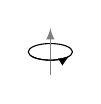
\begin{tikzpicture}
    \draw (0,0) ellipse (.8em and .3em);
    \draw[draw=gray,-latex] (0,-.3) -- (0,+.3);
    \draw[-latex] (0,0) [partial ellipse=210:330:.8em and .3em];
\end{tikzpicture}}}\ \+vE_0 \propto \+ve_1 + i \+ve_2\ {\color{lightgray}\vert} \ {左円偏光}\ \raisebox{-.4em}{\smash{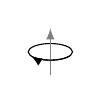
\begin{tikzpicture}
    \draw (0,0) ellipse (.8em and .3em);
    \draw[draw=gray,-latex] (0,-.3) -- (0,+.3);
    \draw[-latex] (0,0) [partial ellipse=330:210:.8em and .3em];
\end{tikzpicture}}}\ \+vE_0 \propto \+ve_1 - i \+ve_2 &&
\end{flalign*}
\midbreak
\begin{flalign*}
    & \mathitem{基本方程式} && \+vk\cdot \+vE = 0,\quad \+vB = \frac{\+vk}{\omega}\times \+vE &&
\end{flalign*}
\end{cheatresume}
\newheader{媒質界面}
\begin{cheatresume}
\mathitem{電場の振幅\wdiv 一般的な場合に}
\begin{flalign*}
    & \begin{array}[t]{@{}ll}
        \displaystyle r_\parallel = \frac{Z_1 \cos\theta_1 - Z_2\cos\theta_2}{z_1 \cos\theta_1 + Z_2 \cos\theta_2} & \displaystyle r_\perp = \frac{Z_2 \cos\theta_1 - Z_1 \cos\theta_2}{Z_2 \cos\theta_1 + Z_1\cos\theta_2} \\[.5em]
        \displaystyle t_\parallel = \frac{2Z_2 \cos\theta_1}{Z_1 \cos \theta_1 + Z_2 \cos\theta_2} & \displaystyle t_\perp = \frac{2Z_2 \cos\theta_1}{Z_2 \cos\theta_1 + Z_1 \cos\theta_2}
    \end{array}
\end{flalign*}
\mathitem{電場の振幅\wdiv $\mu \approx \mu_0$の場合に}
\begin{flalign*}
    & \begin{array}[t]{@{}ll}
        \displaystyle r_\parallel = \frac{\tan\pare{\theta_1 - \theta_2}}{\tan\pare{\theta_1 + \theta_2}} & \displaystyle r_\perp = -\frac{\sin\pare{\theta_1 - \theta_2}}{\sin\pare{\theta_1 + \theta_2}} \\[.5em]
        \displaystyle t_\parallel = \frac{2\cos\theta_1 \sin\theta_2}{\sin\pare{\theta_1 + \theta_2}\cos\pare{\theta_1 - \theta_2}} & \displaystyle t_\perp = \frac{2\cos\theta_1 \sin\theta_2}{\sin\pare{\theta_1 + \theta_2}}
    \end{array}
\end{flalign*}
\mathitem{エネルギー} \quad $\displaystyle R = \abs{\frac{\+un\cdot\expc{\+vS\+_R_}}{\+un\cdot\expc{\+vS\+_I_}}} = \frac{\abs{E\+_0R_}^2}{\abs{E\+_0I_}^2}$ \\
\phantom{\mathitem{エネルギー} \quad }$\displaystyle T = \abs{\frac{\+un\cdot\expc{\+vS\+_T_}}{\+un\cdot\expc{\+vS\+_I_}}} = \frac{Z_1 \cos\theta_2}{Z_2 \cos\theta_1}\frac{\abs{E\+_0T_}^2}{\abs{E\+_0I_}^2}$
\begin{flalign*}
    & \mathitem{{\mysans Brewster}角} && \displaystyle \tan \theta\+_B_ = \frac{n_2}{n_1} &&
\end{flalign*}
\midbreak
\begin{flalign*}
    & \mathitem{全反射} && \sin \theta\+_c_ = \frac{n_2}{n_1} && \\
    & \mathitem{波数} && k\+_T\mathnormal{x}_ = k\+_I\mathnormal{x}_ = k_1 \sin\theta_1 && \\
    & && k\+_T\mathnormal{z}_ = k_1 \sqrt{\pare{n_2/n_1}^2 \sin^2\theta_1} = i\kappa && \\
    & \mathitem{電場} && \+vE\+_T_ = \+vE\+_0T_e^{-\kappa z}e^{i\pare{k_1 \sin \theta_1\, x - \omega t}} && \\
    & \+:c5l{\mathitem{{\mysans Fresnel}関係式に対し}\quad $\begin{array}[t]{l}
        n_2 \sin\theta_2 = n_1 \sin\theta_1,\\ \cos\theta_2 = i\sqrt{\pare{n_1/n_2}^2\sin^2\theta_1 - 1} \\
        R = 1,\quad T = 0
    \end{array}$}
\end{flalign*}
\end{cheatresume}
\columnbreak
\newheader{自由空間における電磁波}
\begin{cheatresume}
\begin{flalign*}
    & \mathitem{電磁場} && \abs{\+vE} = c\abs{\+vB} &&
\end{flalign*}
\midbreak
\begin{flalign*}
    & \mathitem{エネルギー密度} && w = \epsilon_0 E^2 = {B^2}/{\mu_0}, \  \expc{w} = \epsilon_0 \abs{\+vE}^2/2 && \\
    & \mathitem{{\mysans Poynting}ベクトル} && \+vS = \+vE\times \+vH = wc\+uk &&% \\
    %& \mathitem{運動量密度} && \+vg = \epsilon_0 \+vE\times \+vB = \frac{\+vS}{c^2} = \frac{w}{c}\+uk && \\
    %& \mathitem{角運動量密度} && \+vl = \+vr\times \+vg \perp \+vk &&
\end{flalign*}
\end{cheatresume}
\newheader{媒質における電磁波}
\begin{cheatresume}
\begin{flalign*}
    & \mathitem{電磁場} && \abs{\+vH} = {\abs{\+vE}}/{Z},\  Z = \sqrt{{\mu}/{\epsilon}} &&
\end{flalign*}
\midbreak
\begin{flalign*}
    & \mathitem{エネルギー密度} && w = \epsilon E^2 = {B^2}/{\mu},\quad \expc{w} = \epsilon \abs{\+vE}^2/2 && \\
    & \mathitem{{\mysans Poynting}ベクトル} && \+vS = \+vE \times \+vH = \frac{\abs{\+vE_0}^2}{2Z}\+uk
\end{flalign*}
\end{cheatresume}
\newheader{導体界面}
\begin{cheatresume}
\begin{flalign*}
    & \mathitem{複素誘電率} && \tilde{\epsilon} = \epsilon + i\frac{\sigma}{\omega} = \epsilon\pare{1+i \frac{\sigma}{\epsilon\omega}} && \\
    & \mathitem{複素屈折率} && \tilde{n} = c\sqrt{\mu \tilde{\epsilon}} && \\
    & \mathitem{複素抵抗} && \tilde{Z} = \sqrt{\frac{\mu}{\tilde{\epsilon}}} && \\
    & \mathitem{複素波数} && \+vk = \+v\beta + i \+v\alpha && \\
    & && \beta^2 - \alpha^2 = \omega^2\mu\epsilon,\quad 2\+v\alpha\cdot \+v\beta = \omega\mu\sigma &&
\end{flalign*}
\midbreak
\begin{flalign*}
    & \mathitem{電場} && \+vE = \+vE_0 e^{-\+v\alpha\cdot \+vr} e^{i\pare{\+v\beta\cdot \+vr - \omega t}} && \\
    & \mathitem{磁場} && \+vH = \frac{\pare{\+v\beta + i\+v\alpha}\times \+vE}{\omega\mu} &&
\end{flalign*}
\midbreak
\begin{flalign*}
    & \mathitem{反射の法則} && k^{\pare{\mathrm{R}}}_x = k^{\pare{\mathrm{I}}}_x,\quad k^{\pare{\mathrm{R}}}_y = 0,\quad k^{\pare{\mathrm{R}}}_z = -k^{\pare{\mathrm{I}}}_z && \\
    & \mathitem{屈折の法則} && \beta_x = k^{\pare{\mathrm{I}}}_x,\quad \beta_y = 0,\quad \+v\alpha \parallel \+un
    %& && \alpha_x = 0,\quad \alpha_y = 0 \Rightarrow \+v\alpha \parallel \+un &&
\end{flalign*}
\midbreak
\begin{flalign*}
    & \mathitem{良導体} && \frac{\sigma}{\epsilon\omega} \gg 1 \Rightarrow  \alpha \approx \beta \approx \sqrt{\frac{\omega\mu\sigma}{2}} &&
\end{flalign*}
\midbreak
\begin{flalign*}
    & \mathitem{散逸} && \+/\expc{P}/A/ = \frac{\alpha}{2\sigma}\abs{\+v\kappa_0}^2 &&
\end{flalign*}
\midbreak
\begin{flalign*}
    & \mathitem{注意} && \Re \tilde{n} \neq n,\quad \Re \tilde{Z}\neq Z && 
\end{flalign*}
\end{cheatresume}
\columnbreak
\newheader{導波管と共振器}
\begin{cheatresume}
\begin{flalign*}
    & \mathitem{一般境界条件} && \+vE_\parallel \vert_S = 0 \\[-\baselineskip] & && \pare{\div \+vE}_S = 0 \Rightarrow \begin{cases}
        \displaystyle \left.\+DnD{E_n}\right\vert_S = 0 \\% & \mathcomment{平面境界} \\
        \displaystyle \rec{E_r}\left. \+DrD{E_r}\right\vert_{r=R} = -\frac{2}{R} % & \mathcomment{球面境界}
    \end{cases} && \\
    & \mathitem{方程式} && \begin{array}[t]{ll}
        \curl \+vE = i\omega\mu \+vH & \div \+vE = 0 \\
        \curl \+vH = -i\epsilon\omega \+vE & \div \+vH = 0
    \end{array} &&\\
    & && \+vE \rightarrow \+vH,\quad \+vH \rightarrow -\+vE, \quad \epsilon \leftrightarrow \mu  &&
\end{flalign*}
\midbreak
\begin{flalign*}
    & \mathitem{導波管} \\
    & \mathitem{一般解} && \+vE\pare{\+vr,t} = \+vE\pare{x,y}e^{i\pare{kz-\omega t}} && \\
    & && \+vH\pare{\+vr,t} = \+vH\pare{x,y}e^{i\pare{kz-\omega t}} && \\
    & \mathitem{電磁場} && \begin{array}[t]{@{}lll}
        \mathitem{TM} & \pare{\laplacian_t + \gamma^2} E_z = 0 & \displaystyle \+vE_t = \frac{ik}{\gamma^2}\grad_t E_z \\ & \+:c2{l}{\displaystyle \+vH_t = \frac{\omega\epsilon}{k}\+uz\times \+vE_t} \\
        \mathitem{TE} & \pare{\laplacian_t + \gamma^2} H_z = 0 & \displaystyle \+vH_t = \frac{ik}{\gamma^2}\grad_t H_z \\ & \+:c2{l}{\displaystyle \+vE_t = -\frac{\omega\mu}{k}\+uz\times \+vH_t} \end{array} && \\
    & \mathitem{境界条件} && \begin{array}[t]{@{}lll}
        \mathitem{TM} & H_z \equiv 0 & E_z\vert_S = 0 \\
        \mathitem{TE} & E_z \equiv 0 & \displaystyle  \left.\+DnD{H_z}\right\vert_S = 0 
    \end{array} && \\
    & \mathitem{波数} && \gamma^2 = \mu\epsilon\omega^2 - k^2 &&
\end{flalign*}
\midbreak
\begin{flalign*}
    & \mathitem{矩形導波管} && \mathrm{TE}_{10}, \mathrm{TE}_{01}, \mathrm{TE}_{11}, \mathrm{TM}_{11},\cdots \\
    & \mathitem{TM} && E_z = E_0 \sin \frac{m\pi x}{a} \sin \frac{n\pi y}{b} \\
    & \mathitem{TE} && H_z = H_0 \cos \frac{m\pi x}{a} \cos \frac{n\pi y}{b}\\ & && \gamma_{mn}^2 = \pi^2\pare{\frac{m^2}{a^2} + \frac{n^2}{b^2}}\\ & && \omega_{mn} = c\sqrt{\pare{\frac{\pi m}{a}}^2 + \pare{\frac{\pi n}{b}}^2 + k^2} &&
\end{flalign*}
\midbreak
\begin{flalign*}
    & \mathitem{共振器} && E_x = A_1 \cos k_1 x \sin k_2 y \sin k_3 z e^{-i\omega t} && \\
    & && E_y = A_1 \sin k_1 x \cos k_2 y \sin k_3 z e^{-i\omega t} && \\
    & && E_z = A_1 \sin k_1 x \sin k_2 y \cos k_3 z e^{-i\omega t} && \\
    & && k_x = {m\pi}/{L_x},\quad k_y = {n\pi}/{L_y},\quad k_z = {l\pi}/{L_z} && \\
    & && \omega = ck \mathcomment{$m,n,l\neq 0$高々1つを除く} &&
    %& && \omega = c\sqrt{\pare{\frac{m\pi}{L_x}}^2 + \pare{\frac{n\pi}{L_y}}^2 + \pare{\frac{l\pi}{L_z}}^2} &&
\end{flalign*}
\end{cheatresume}
\end{multicols*}

\end{document}
